\chapter{Introduction to the Mandelbrot Set}
We consider the set of quadratic polynomials \( \{f_c(z)=z^2+c:c\in \mathbb{C}\} \). It is
enough to consider this set because every quadratic polynomial is linearly conjugate to a quadratic
polynomial of the type \( f_c(z) \) for some unique \( c\in \mathbb{C} \).

To prove this, let \( f(z)=pz^2+qz+r \), \( p\neq 0 \). Consider the conjugation with
the map, \( \sigma(z)=az+b \) with \( a=p \) and \( b=q /2 \). Then, we have
\begin{align*}
	\sigma f \sigma^{-1}(z)&=a\left(p\left(\frac{z-b}{a}\right)^2+q\left( \frac{z-b}{a}\right) +r  \right)+b\\
						   &=(z-b)^2+q(z-b)+ar+b\\
						   &=z^2+b^2-qb+ar+b\\
						   &=z^2+q^2 /4-q^2 /2+pr+q /2\\
						   &=z^2+(pr+q /2-q^2 /4)
.\end{align*}
This is of the form \( z^2+c \) for \( c=pr+q /2-q^2 /4 \).

\section{Definition of the Mandelbrot Set}
First, we define as new type of set, known as the \emph{Filled-in Julia Set} for a polynomial \( P \).

\begin{definition}[Filled-in Julia Set]
The Filled-in Julia Set of a polynomial \( P \)	is defined as \( K(P)=\Cinf\bs F_\infty(P) \). It
is the union of the Julia set and the bounded Fatou components.
It is denoted by \( K(P) \) or simply \( K \) when the context is clear.
\end{definition}
\noindent By \Cref{lem1.2}, \( K \) can also be defined as follows:\[
	K=\{z\in \mathbb{C}:\pop[n](z)\text{ is bounded}\}
.\] 

\noindent \textbf{Notation.} We will use \( F_c \), \( J_c \) and \( K_c \) for the 
\( F_\infty(f_c) \), \( J(f_c) \) and \( K(f_c) \) respectively.

\begin{definition}[\textbf{Mandelbrot Set}]
	The Mandelbrot Set is defined as \[ 
	M=\{c\in \mathbb{C}:K_c \text{ is connected}\}. 
\]
\end{definition}

\noindent Now, we have the following two theorems for polynomials:
\begin{itemize}
\item For polynomials, since \( F_\infty \) is a completely invariant Fatou component 
	(by \Cref{thm1.4}), \( \partial F_\infty=J \) (by \Cref{thm1.2}).
\item And, from \Cref{thm1.1}, we have that \( F_\infty \) is simply connected \( \iff \)
	\( \Cinf\bs F_\infty \) is connected \( \iff \) \( \partial F_\infty \) is connected.
\end{itemize}
Thus, for a polynomial,\[
	F_\infty \text{ is simply connected } \iff K \text{ is connected } \iff J \text{ is connected}
.\]

\noindent Hence, we have the following equivalent descriptions for the Mandelbrot Set:
\begin{align*}
	M &=\{c\in \mathbb{C}:K_c \text{ is connected}\}\\
	  &=\{c\in \mathbb{C}:F_c \text{ is simply connected}\}\\
	  &=\{c\in \mathbb{C}:J_c \text{ is connected}\}
.\end{align*}

\section{The Fundamental Dichotomy}
\begin{theorem}
	For a polynomial \( P \), the following are equivalent:
	\begin{enumerate}
		\item \( F_\infty \) is simply connected \( \iff \) \( J \) is connected \( \iff \) \( K \) is connected.
		\item There are no finite critical points of \( P \) in \( F_\infty \).
	\end{enumerate}
\end{theorem}
\begin{proof}
	First assume that \( F_\infty \) is simply connected \( \implies c(F_\infty)=1 \) and hence, \( \chi(F_\infty)=2-c(F_\infty)=1 \).
	Now, since \( F_\infty \) is completely invariant and \( P \) is a polynomial of degree \( d \) (say), \( P \) is a \( d \)-fold
	map of \( F_\infty \) onto itself.
	Applying the Riemann-Hurwitz relation to the map \( P \) of \( F_\infty \) onto itself, we obtain,
	\begin{align*}
		&\chi(F_\infty)+\delta_P(F_\infty)=d\,\chi(F_\infty)\\
		\implies & 1+\delta_P(F_\infty)=d\\
		\implies & \delta_P(F_\infty)=d-1
	.\end{align*}
	Now, \( \delta_P(\infty)=d-1 \) and therefore, \( P \) does not have any finite critical points in \( F_\infty \).

	For the converse part, assume there are no critical points of \( P \) in \( F_\infty \). Then, the Bottcher's map \( \phi \) which
	conjugates \( P \) to the map, \( z\mapsto z^d \) can be extended to the whole of \( F_\infty \) and \( \phi:F_\infty\to \mathbb{D} \)
	is a biholomorphism. Hence, \( F_\infty \) is simply connected.
\end{proof}

Now, quadratic maps have only one finite critical point and \( f_c \) have the critical point at \( 0 \) for all \( c\in \mathbb{C} \).
Hence, by the Fundamental Dichotomy, \( F_c \) is simply connected \( \iff \) \( 0\not\in F_c \) or \( 0\in K_c \). Using, \( c_n \) to denote \( \fcof[n](0) \),
we get,
\begin{align*}
	M&=\{c\in \mathbb{C}:0\in K_c\}\\
	 &=\{c\in \mathbb{C}:(c_n)\text{ is bounded}\}
.\end{align*}
Note that \( c_0=0 \) and \( c_1=f_c(0)=c \). So, \( (c_n) \) is also the forward orbit of \( c \). Hence, in other words,
the Mandelbrot Set consists of \( c\in \mathbb{C} \) such that its forward orbit under the map \( f_c \)
remains bounded.

\section{The other end of the Dichotomy Theorem}
By the Dichotomy Theorem, we can say that if even one finite critical point of \( P \) lies in \( F_\infty \), then \( K \)
cannot be connected. But this theorem states that if all finite critical points of \( P \) lie in \( F_\infty \), then
\( K \) is not only disconnected, but totally disconnected.

\begin{definition}[Cantor set]
	A subset \( X\subset \Cinf \) is called a Cantor set if it is non-empty, closed, perfect and totally disconnected.
\end{definition}

\begin{theorem}
	Let \( R \) be a rational map with \( \deg(R)\ge 2 \). Let \( \alpha \) be a super-attracting fixed
	point of \( R \). If the Fatou component of \( R \) containing \( \alpha \), say \( F_\alpha \),
	contains all the critical points of \( R \), then \( J(R) \) is a Cantor set.
\end{theorem}

\begin{corollary}
	If \( c\not\in M \), then \( J_c \) is a Cantor set.
\end{corollary}
\begin{proof}
	Since \( 0 \) is the only critical points of \( f_c \) (apart from \( \infty \)), if it belongs to \( F_c=F_\infty(f_c) \), 
	i.e. if \( 0\not\in K_c \iff c\not\in M \), then \( J_c \) is a Cantor set.
\end{proof}

\section{Some properties of the Mandelbrot Set}
We know, \( M=\{c\in \mathbb{C}:(c_n)\text{ is bounded}\} \). 
This description for \( M \) can be strengthened significantly by the following theorem:
\begin{theorem}\label{thm4.1}
	\( M=\{c\in \mathbb{C}:|c_n|\le 2 \}.\)
\end{theorem}
\begin{proof}Obviously, \( \{c\in \mathbb{C}:|c_n|\le 2\}  \subseteq M\).

	Now, Suppose that \( c\in M \). We need to prove that \( |\fcof[n](c)|=|c_n|\le 2 \) for all \( n\in \mathbb{N} \).\\
	Consider the set \( W_c=\{z\in \mathbb{C}:|z|\ge |c|,|z|>2\} \). For \( z\in W_c \),\[
		|f_c(z)|=|z^2+c|\ge |z|^2-|c|\ge |z|^2-|z|\ge |z|(|z|-1)=|z|(1+\epsilon)
	\] for some \( \epsilon>0 \) (as \( |z|>2 \)). Clearly, \( |\fcof[n](z)|\ge |z|(1+\epsilon)^n \implies z\not\in K_c\).\\
	This implies \( |c|\le 2 \). Consequently, \( |\fcof[n](c)|\le 2 \) for all \( n\in \mathbb{N} \).\\
	Hence, \( M\subseteq  \{c\in \mathbb{C}:|c_n|\le 2 \} \).

	Therefore, \( M=\{c\in \mathbb{C}:|c_n|\le 2\} \).
\end{proof}

As \( c_1=c \), we have that \( |c|\le 2 \) for all \( c\in M \) i.e \( M \subseteq \{c\in \mathbb{C}:|c|\le 2\} \). 
This turns out to be the strongest bound possible for \( |c| \)
as \( -2\in M \). The orbit of \( 0 \) under the map \( z\mapsto z^2-2 \) is: \[ 0\mapsto -2\mapsto 2\mapsto 2 \]
and hence is bounded.

\begin{theorem}
	The Mandelbrot set \( M \) is compact and \( \Cinf\bs M \) is open and connected.
\end{theorem}
\begin{proof}
	Let, \( c_n=\fcof[n](c)=Q_n(c) \) be a polynomial in \( c \). Clearly, from \Cref{thm4.1} \[
		M=\cap_{n=1}^{\infty}Q_n^{-1}(\overline{\mathbb{D}_2}),
	\] where \( \overline{\mathbb{D}_2}=\{z\in \mathbb{C}:|z|\le 2\} \).
	Thus, \( M \) is closed. It is already known that it is bounded. Hence, it is compact.

	Now, \[
		\Cinf\bs M=\cup_{n=1}^\infty Q_n^{-1}(E)
	\] where \( E=\Cinf\bs\overline{\mathbb{D}_2}\). Now, \( E \) is open and connected and 
	since, \( Q_n \) are non-constant polynomials, \( Q_n^{-1}(E) \) is open and connected for all \( n\in \mathbb{N} \).
	Also, each one of them contains \( \infty \) and hence, their union is also open and connected.\\
	Therefore, \( \Cinf\bs M \) is open and connected.

\end{proof}

\section{Plotting the Mandelbrot Set}
\Cref{thm4.1} is also used to plot the Mandelbrot Set. A simple code would involve going through each
pixel \( (x,y) \) in a \( N\times N \) square (where \( N>2 \)) and seeing if the iterates of \( 0 \)
under the map, \( f_c(z)=z^2+c \), where \( c=x+iy \),
become larger than of modulus \( 2 \) after a large number of iterations.

If the modulus of iterates of \( 0 \) do not cross the value \( 2 \) after a large number of iterations,
\( c=x+iy \) probably lies in the Mandelbrot set and we color it black. If not, then we leave it uncolored.

A simple code in Python generates the following picture:

\begin{figure}[htbp]
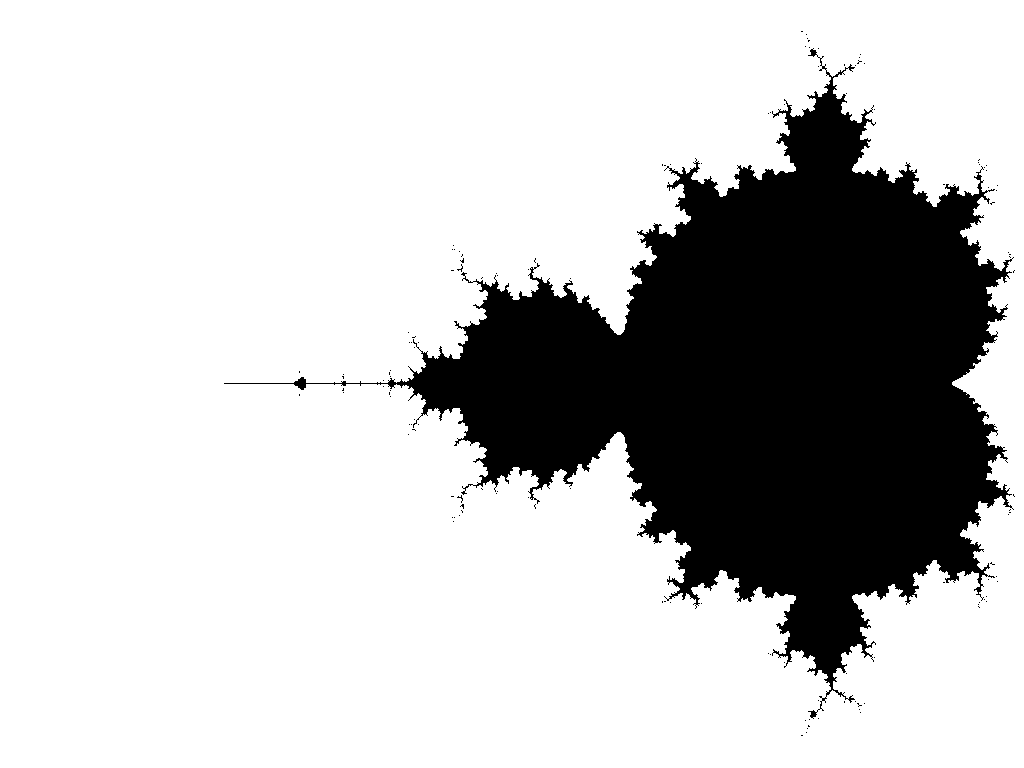
\includegraphics[scale=.35]{figures/mandelbrot.png}
\caption{The Mandelbrot Set}
\label{mandelbrot}
\end{figure}
